\chapter{A LIBRARY FOR LOCAL DIFFERENTIAL PRIVACY}

\section{Introduction in Local DP}

As we mentioned in previous chapters, there are two major forms of Differential Privacy. Having analyzed and tested the first one, \textbf{Global D.P.}, it is now time to examine \textbf{Local D.P.}, by explaining some possible protocols, as well as building our own.


In Local D.P., there is a significant difference compared to Global DP: there is \textbf{no trusted curator} between the data and the users, as they just want to send their data, while already being anonymized. Thus, an algorithm must perturb the data before sending it to the untrusted curator, who will then transmit it to the analysts. 

In order to achieve that goal, the user must randomize the value before making it public (i.e. sending it to the untrusted curator). Then, the curator which collects the data (we will reference to him as aggregator moving forward), collects the data and tries to retrieve their original values, with a goal of producing the most accurate results possible. 

Thus, each LDP algorithm has the following steps:

\begin{itemize}
    \item Each user encodes, and then perturbs the private value that he wants to make public
    \item Each user sends out the result of the perturbation process, with that being only the final value, as they keep the intermediate results for themselves
    \item The untrusted data curator collects each user's value, and implements some kind of aggregation in order to retrieve the stats that he wants from the data given to him.
\end{itemize}

In comparison with Global D.P., the Local model has advantages, as well as disadvantages. 
Its main advantages are:
\begin{itemize}
    \item The user is not forced to trust the data curator, as only the perturbed value is reported
    \item Simpler implementation of the algorithms, due to the district steps taken by both sides.
\end{itemize}

while the main disadvantages are the following:

\begin{itemize}
    \item The noise added should be larger than the Global model, in order to satisfy the definition, thus the number of people in the dataset should be significant for accurate results to be produced.
    \item Because this is not always possible, many real-world applications use extremely high values of epsilon compared to what we got used to during our testing in the Global models.
\end{itemize}

During this Thesis, concern was raised for the main disadvantage of L.D.P., and thus\textbf{ we will present a new protocol aiming to reduce the need for many users, while still covering the definition.} However, the definition for L.D.P. is quite different than the Global model one's.

\section{Definition of Local DP}

Having a general idea in how Local D.P. functions, it is now time to give a strict definition that we are going to depend our work on moving forward.

We can say that an algorithm $A$ satisfies ε-Local Differential Privacy, if and only if for any input $v_1$, $v_2$, we have

$$ \forall y \in Range(A):\ Pr[A(v_1) = y] \leq e^{\epsilon} * Pr[A(v_2) = y] $$

where $Range(A)$ denotes the set of all possible outputs of the algorithm $A$.

As mentioned in Chapter 2, this definition can have many interpretations by different algorithms or protocols, but each one must produce a probabilistic space whose elements must satisfy the above equation.


\section{Simple Application of LDP}

The most simple of L.D.P. protocols is already mentioned in this Thesis, and is no other than the \textbf{Randomized Response} protocol. This algorithm implements the three steps mentioned in the introduction, as the user chooses a value (Yes or No), perturbs it (by the flipping of the coins), reports the perturbed value, with the sole job of the aggregator being to collect, normalize and report the values provided. It meets the definition of L.D.P., as the fraction of a pair of probabilities in the space of possible outputs (Yes, No) has always the ceiling of a real number. 

Our goal is to now find this ceiling, and thus denote the level of privacy that randomized response offers. In order to do this, we are going to select the possibility of the user having chose the answer "Yes". A simple case analysis shows that $Pr[Yes | Truth] = \frac{3}{4}$, and of course $Pr[Yes | False] = \frac{1}{4}$. Thus, by the definition of L.D.P., we have 

\begin{align*}
    \frac{Pr[Yes | Truth]}{Pr[Yes | False]} = \frac{\frac{3}{4}}{\frac{1}{4}} = 3 = e^\epsilon \Longleftrightarrow \epsilon = ln(3)
\end{align*}

Thus, R.R. offers  $ln(3)$-differential privacy to its users. This is quite a good setting, but the restriction is that the user can only report 2 values, something not suitable for modern problems and surveys. 

However, having implemented R.R. in Python, we can now display the accuracy error of R.R. as the number of users rises.

In R.R., we care about the total true answers of the users, and not the individual responses. Thus the metric we are going to use is the \textbf{absolute difference of the sum of the 2 vectors: the one with the truthful answers, and the one with the reported answers}. We are going to divide this result with the number of the users, in order to get the scale of the error depending on the size of the vector that was reported. The metric is expressed from the following function:

\begin{align*}
    Error = \frac{abs(sum(true\_values) - sum(reported\_values)) }{number\ of \ users}
\end{align*}

As always, during the creation of probabilistic distributions, one run is not enough, because of the extreme amount of noise that can occur. Thus, for each number of users we are going to run the R.R. protocol 100 times, and the final accuracy error will be produced by the mean value of those runs.

The results of the testings are shown bellow in \textbf{Figure 4.1}.

\begin{figure}[!htb]\centering
    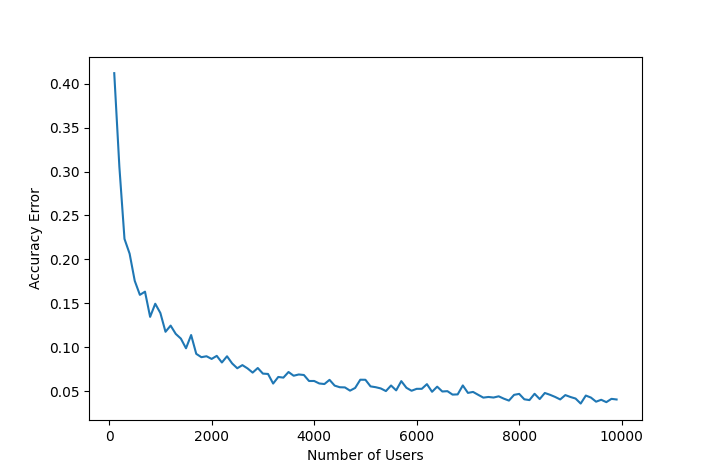
\includegraphics[width=0.8\textwidth]{images/rr_results.png}
    \caption{Accuracy Error in R.R for increasing values of epsilon}
\end{figure}


We observe that the plot behaves as expected: the protocol produces a logarithmic curve for the accuracy error, while for a large number of users (over 3000), the error stabilizes bellow $0.1$. 